\chapter{Réseaux de régulation génétique et graphes d'interaction}
\label{rrg}
Afin de permettre la modélisation des interactions entre gènes malgré le peu de données disponibles, René Thomas propose en 1973 un outil basé sur l'utilisation de booléens au sein d'un graphe d'interactions. Cependant, ce modèle s'avère trop simpliste, et Thomas l'étend entre 1990 et 2000 en un modèle qui permet l'attribution de plusieurs niveaux d'expression aux gènes \cite{richard-comet-bernot-08}. Ce modèle sera développé au sein de ce chapitre. Il fera l'objet d'une présentation en termes intuitifs dans l'introduction, puis sera redéfini de façon formelle dans les sections suivantes.

\section{Introduction}
Le modèle présenté ici repose en premier lieu sur l'élaboration d'un graphe orienté, appelé dans ce contexte \emph{graphe d'interaction}. Un tel graphe représente un ensemble de gènes, qui peuvent s'influencer mutuellement (positivement ou négativement). Les gènes sont intuitivement modélisés par les n\oe uds du graphe, tandis que les interactions sont représentées par les arcs reliant ces n\oe uds, et dont l'étiquette précise le type d'influence. Un gène n'est en mesure d'influencer d'une certaine manière (par exemple : positivement) un autre gène (ou de s'influencer lui-même) que si son niveau d'expression est suffisant ; dans le cas inverse, il aura l'influence contraire (une influence négative si on suit le même exemple).

Dans ce type de modélisation, le niveau d'expression d'un gène est directement lié à la quantité (ou la concentration) de protéine codée par ce gène qui est présente dans le milieu. Cependant, comme mentionné au paragraphe précédent, les données disponibles sont très lacunaires, et le niveau d'expression nécessaire pour qu'un gène exerce une influence sur un autre (aussi appelé \emph{seuil d'activation}) n'est généralement pas connu. Pour combler cette insuffisance de données, le niveau d'expression d'un gène n'est pas représenté directement par la quantité de protéine codée, mais par un nombre fini de niveaux discrets, de façon à ce que si le niveau d'expression d'un gène est connu à un instant donné, on peut immédiatement déterminer quel est le niveau d'influence que ce gène exerce sur toutes ses cibles dans le graphe d'interactions. Le nombre de niveaux d'expression différents accessibles pour un gène peut donc au plus être égal au nombre de gènes sur lesquels il peut potentiellement avoir une influence. Un exemple de graphe d'interaction est donné à la figure~\ref{rrg-gi-sans-multiplexe}.\\

\begin{figure}[ht]
  \centering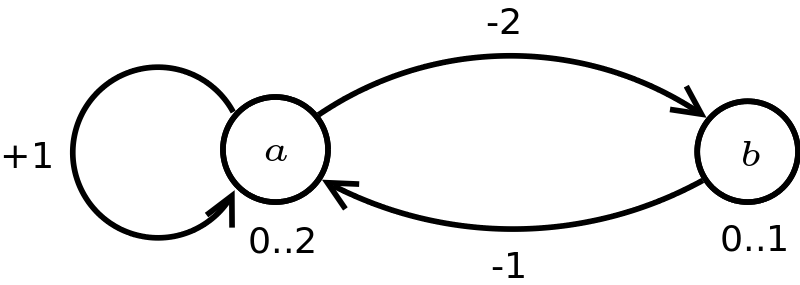
\includegraphics[width=7cm]{figs/gi-sans-multiplexe}
  \caption{Un exemple de graphe d'interaction simple \cite{richard-comet-bernot-08} : les n\oe uds modélisent les gènes et les arcs leurs influences mutuelles. Ici, le gène $a$ s'auto-active tandis que les deux gènes $a$ et $b$ s'inhibent mutuellement. Les valeurs sous les n\oe uds indiquent les niveaux d'expressions accessibles pour chaque gène.}
  \label{rrg-gi-sans-multiplexe}
\end{figure}

Dans le modèle originellement proposé par Thomas, un gène pouvant potentiellement exercer une influence sur un autre gène est relié à celui-ci par un arc (dirigé vers ce dernier) étiqueté par une valeur de seuil et un type d'influence (qui consiste en une information booléenne car l'influence ne peut être que positive ou négative). Ainsi, pour savoir si ce gène exerce son influence sur le second gène à un instant donné, il suffit de comparer le niveau d'expression de ce gène à cette valeur de seuil, à l'aide d'une simple relation d'inégalité : une interaction positive (resp. négative) ne pourra avoir lieu que si le niveau d'expression du gène est supérieur (resp. inférieur) au seuil. Les assertions qui conditionnent les influences entre gènes consistent donc uniquement en des inégalités.

Si ce modèle permet de représenter une grande partie des relations d'influences des systèmes étudiés, il subsiste cependant des cas pour lesquels il échoue à représenter certains comportements. On peut notamment citer le cas où plusieurs gènes doivent s'associer pour exercer une influence ; ce cas ne peut pas être représenté car les arcs d'un graphe d'interaction ne peuvent partir que d'un unique n\oe ud, pour n'arriver que dans un unique n\oe ud. De même, on pourrait imaginer une situation où un gène peut exercer une influence sur un autre lorsque son niveau d'expression \og n'est pas trop élevé \fg, et qu'il se trouve donc dans un intervalle ; à nouveau, les inégalités simples ne permettent pas de prendre ce type de comportement en compte.

Afin de combler cette lacune, la notion de \emph{multiplexe} a été proposée pour de permettre la modélisation de comportements plus complexes \cite{bernot-comet-khalis-08, khalis-bernot-comet-richard-roux-siebert-UnPublished}. Les multiplexes viennent s'ajouter aux étiquettes des arcs du modèle présenté précédemment. Ils se présentent comme des n\oe uds d'un type différent de ceux représentant les gènes au sein du graphe d'interactions, et comportent :
\begin{itemize}
  \item un nom,
  \item une assertion, appelée \emph{condition d'influence}, exprimée en logique modale et qui dépend uniquement de ses prédécesseurs dans le graphe (gènes ou autres multiplexes).
\end{itemize}
Ainsi, un gène pouvant potentiellement exercer une influence sur un autre possède un arc sortant qui pointe vers un multiplexe, et ce multiplexe possède à son tour un arc sortant pointant vers le gène final. L'influence aura effectivement lieu si la condition d'influence du multiplexe est satisfaite. Dans ce modèle, on permet qu'un multiplexe possède un arc sortant vers un autre multiplexe, à condition qu'il n'existe pas de cycle ne faisant intervenir que des multiplexes. La figure~\ref{rrg-gi-avec-multiplexe} reprend l'exemple précédent en le complétant avec les multiplexes correspondants.

\begin{figure}[ht]
  \centering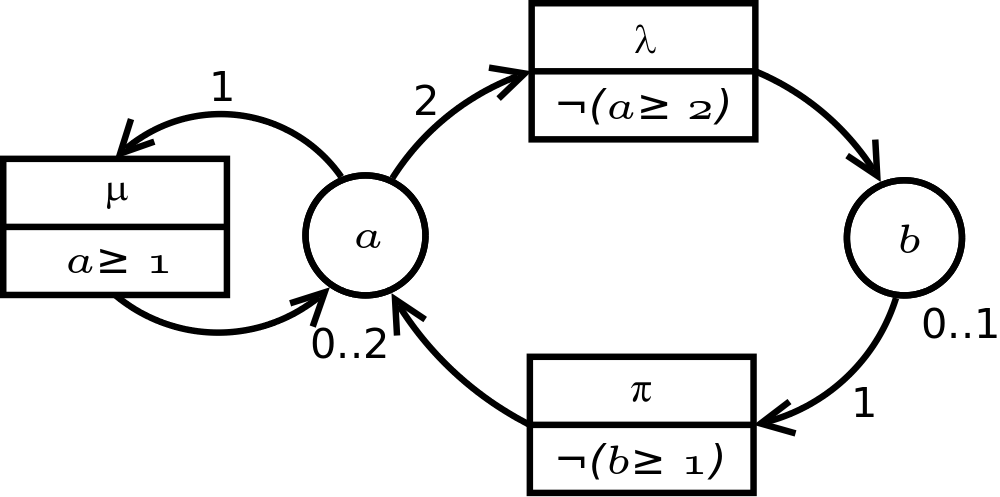
\includegraphics[width=7cm]{figs/gi-avec-multiplexe}
  \caption{Un exemple de graphe d'interaction avec multiplexes : les conditions d'influence sont précisées dans un nouveau type de n\oe ud appelé multiplexe. Pour comparaison, ce graphe définit exactement le même système de gènes que celui de la figure~\ref{rrg-gi-sans-multiplexe}.}
  \label{rrg-gi-avec-multiplexe}
\end{figure}

\section{Graphe d'interaction et paramétrisation}
Définissons le modèle du graphe d'interaction de façon formelle, d'après la description de la partie précédente. Il est à noter que les n\oe uds du graphe d'interaction représentant les gènes sont appelés \emph{variables}. Dans la suite, on utilisera les deux dénominations, bien que le terme de \emph{gène} semble plus adapté à une description biologique des phénomènes mis en jeu.
\begin{definition}[Graphe d'interaction]
Un \emph{graphe d'interaction avec multiplexes} est un quadruplet $G = (V ; M ; E_V ; E_M)$ qui vérifie les propriétés suivantes :
\begin{itemize}
  \item $(V \cup M ; E_V \cup E_M)$ est un graphe orienté et étiqueté, dont les n\oe uds sont $V \cup M$ et les arcs sont $E_V \cup E_M$, vérifiant les contraintes suivantes :
  \begin{itemize}
    \item les ensembles $V$ et $M$ sont finis et disjoints ; les éléments de $V$ sont appelés \emph{variables} et ceux de $M$ sont appelés \emph{multiplexes},
    \item les arcs de $E_V$ ont pour source une variable et pour cible un multiplexe, tandis que les arcs de $E_M$ ont pour source un multiplexe et pour cible une variable ou un autre multiplexe,
    \item tout cycle de $G$ contient au moins une variable,
  \end{itemize}
  \item toute variable $v$ de $V$ est étiquetée par un entier positif $b_v$ qui est appelé son \emph{plafond},
  \item tout arc de $E_V$ est étiqueté par un entier positif $s$ inférieur ou égal au plafond de sa variable source et appelé \emph{seuil} ; on note un tel arc $v \xrightarrow{s} m$ où $v$ est sa variable source et $m$ est son multiplexe cible.
  \item tout multiplexe $m$ de $M$ est étiqueté par une formule $\varphi_m$ appartenant au langage $\mathcal{L}_m$ défini inductivement par :
  \begin{itemize}
    \item si $v \xrightarrow{s} m$ appartient à $E_V$ alors $v \geq s$ est un atome de $\mathcal{L}_m$,
    \item si $m' \xrightarrow{} m$ appartient à $E_M$ alors $m'$ est un atome de $\mathcal{L}_m$,
    \item si $\varphi$ et $\psi$ appartiennent à $\mathcal{L}_m$ alors $\neg \varphi$, $\varphi \wedge \psi$ et $\varphi \vee \psi$ sont des atomes de $\mathcal{L}_m$.
  \end{itemize}
\end{itemize}
\end{definition}
On retrouve dans cette définition tous les éléments développés en introduction. Il est à noter que l'introduction de multiplexes ne supprime pas totalement les étiquettes déjà présentes sur les arcs partant des variables. En effet, si l'information concernant le type d'influence (activation ou inhibition) est ici portée par l'assertion du multiplexe, il est en revanche toujours nécessaire de connaître le seuil au delà duquel le niveau d'expression du gène jouera un rôle dans cette assertion.

Afin de pouvoir étudier le comportement d'un système modélisé grâce à l'outil développé ici, il est nécessaire d'introduire une certaine forme de dynamique. Cette notion était déjà présente durant toute la partie d'introduction, lorsqu'il était question des niveaux d'expression des différents gènes (mesurés à partir de la quantité de protéine produite et présente dans le milieu). L'état d'un graphe d'interaction se définit alors aisément comme l'ensemble des niveaux d'expression des variables qui le composent.
\begin{definition}[État d'un graphe d'interaction]
Un \emph{état} d'un graphe d'interaction $G = (V ; M ; E_V ; E_M)$ est une fonction $\eta : V \rightarrow \mathbb{N}$ telle que pour toute variable $v$ de $V$, on ait : $\eta(v) \leq b_v$. $\eta(v)$ est appelé le \emph{niveau d'expression} de $v$.
\end{definition}

Il est important de noter que si l'état d'un graphe d'interaction représente l'état des gènes qui le composent à un instant donné, la notion de temps n'intervient cependant à aucun moment dans le modèle. En effet, la dynamique du graphe d'interactions est vue comme une succession d'instants, mais il n'est en aucun cas question de quantifier la durée qui sépare deux de ces instants. On fera d'ailleurs dans la partie suivante l'hypothèse selon laquelle une durée suffisamment longue s'écoule entre deux changements d'état successifs du graphe.

Pour terminer cette première partie concernant les graphes d'interaction, il nous faut formaliser les possibilités d'influence entre les variables au travers des multiplexes. Dans un état donné, un gène reçoit une influence d'un certain nombre d'autres gènes \textit{via} certains multiplexes. Plus précisément, ces multiplexes doivent posséder un arc sortant vers le gène en question, et leur assertion doit être satisfaite. On parvient donc à la définition suivante, où la notation $G^{-1}(x)$ représente l'ensemble des prédécesseurs d'un n\oe ud $x$ du graphe.
\begin{definition}[Ressources d'une variable]
Étant donnés un graphe d'interaction $G = (V ; M ; E_V ; E_M)$ et un état $\eta$ de $G$, l'ensemble des \emph{ressources} d'une variable $v$ de $V$ pour l'état $\eta$, qu'on note $\rho(v, \eta)$, est l'ensemble des multiplexes $m$ de $G^{-1}(v)$ tels que $\varphi_m$ est satisfaite. L'interprétation de la formule $\varphi_m$ d'un multiplexe $m$ est inductivement définie par :
\begin{itemize}
  \item si $\varphi_m$ est réduite à un atome $v \geq s$, où $v \in G^{-1}(m)$ et $(v \xrightarrow{s} m) \in E_V$, alors $\varphi_m$ est satisfaite ssi $\eta(v) \geq s$,
  \item si $\varphi_m$ est réduite à un atome $m' \in M$, où $m' \in G^{-1}(m)$, alors $\varphi_m$ est satisfaite ssi $\varphi_{m'}$,
  \item si $\varphi_m$ est une formule constituée d'atomes et de connecteurs logiques, alors :
  \begin{itemize}
    \item $\varphi_m \equiv \neg \psi$ est satisfaite ssi $\psi$ n'est pas satisfaite,
    \item $\varphi_m \equiv \psi_1 \wedge \psi_2$ est satisfaite ssi $\psi_1$ et $\psi_2$ sont satisfaites,
    \item $\varphi_m \equiv \psi_1 \vee \psi_2$ est satisfaite ssi $\psi_1$ est satisfaite ou $\psi_2$ est satisfaite.
  \end{itemize}
\end{itemize}
\end{definition}
Le symbole $\equiv$ utilisé dans cette définition et dans les définitions à venir indique l'équivalence entre deux assertions.

\section{Réseau de régulation et graphe d'états asynchrone}
\label{rrg-reseau-de-regulation}
Si la notion d'interaction a largement été abordée jusqu'ici, il n'a pas encore été question de quantifier cette interaction. En effet, si on peut modéliser le fait qu'un gène possède une influence sur un autre gène, car faisant partie de ses ressources, et pouvant donc contraindre ce dernier à changer de niveau d'expression, le modèle actuel ne contient pas d'information quant au niveau vers lequel le gène influencé sera attiré. Il reste donc à définir une \og carte \fg{} des interactions spécifiant, selon les ressources d'une variable, l'état vers lequel celle-ci sera attirée.
\begin{definition}[Réseau de régulation]
Un \emph{réseau de régulation génétique avec multiplexes} est un couple $(G ; \mathcal{K})$ où :
\begin{itemize}
  \item $G = (V ; M ; E_V ; E_M)$ est un graphe d'interaction,
  \item $\mathcal{K} = \{k_{v, \omega}\}$ est une famille de paramètres indexés par $v \in V$ et $\omega \subset G^{-1}(v)$ telle que chaque $k_{v, \omega}$ de $\mathcal{K}$ soit un entier vérifiant : $0 \leq k_{v, \omega} \leq b_v$.
\end{itemize}
$\mathcal{K}$ est appelée \emph{paramétrisation} de $G$ (ou de $N$).
\end{definition}

Le réseau de régulation, extension du graphe d'interaction, est un outil complet comprenant toutes les informations concernant le système étudié et sa dynamique. Il est important de noter qu'il n'existe pas une unique paramétrisation pour un graphe d'interaction donné. En général, le nombre de paramétrisations possibles est très important et constitue l'une des limitations de ce modèle \cite{richard-comet-bernot-08}. Cependant, nous ne nous intéresserons pas dans ce chapitre à leur recherche et travaillerons avec des paramétrisations données. La figure~\ref{rrg-ex-parametrisation} donne un exemple de paramétrisation pour le graphe donné en exemple plus haut.\\

\begin{figure}[htbp]
  %\begin{center}
  \centering%\begin{tabular}{ccc}
  %\leavevmode
  %\subfloat[Graphe d'interaction]{
    \begin{tabular}{c}
      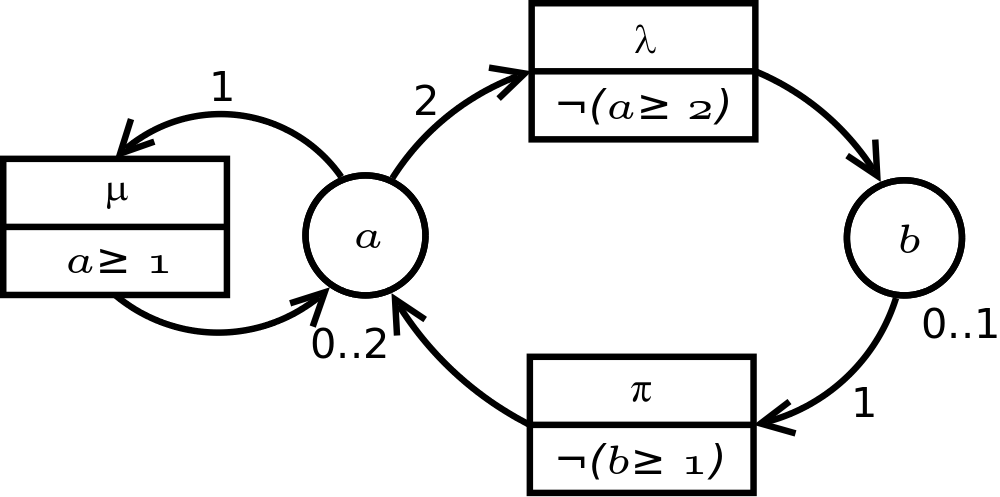
\includegraphics[width=7cm]{figs/gi-avec-multiplexe}
      \\\small(a)
    \end{tabular}
%}
\hspace{.5cm} %&%&
    \begin{tabular}{c}
  %\subfloat[Paramétrisation]{
  %\begin{tabular}[b]{cc}
    $\begin{array}{c|c}
      \omega & k_{a, \omega}\\
      \hline
      \emptyset & 2\\
      \{\mu\} & 2\\
      \{\pi\} & 0\\
      \{\mu, \pi\} & 0
    \end{array}$\hspace{.5cm}%&
    $\begin{array}{c|c}
      \omega & k_{b, \omega}\\
      \hline
      \emptyset & 1\\
      \{\lambda\} & 0
    \end{array}$%\end{tabular}%}
    \\\small(b)
    \end{tabular}
%}  %\end{tabular}
%  \subfloat[test]{
%    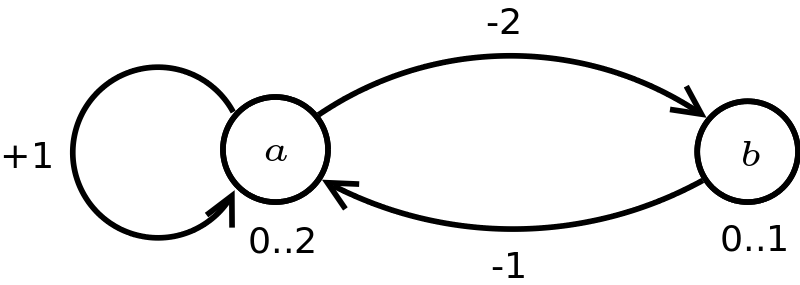
\includegraphics[width=7cm]{figs/gi-sans-multiplexe}} %&
  %\end{center}
  \caption{Un exemple réseau de régulation génétique comprenant un graphe d'interaction (a) et une paramétrisation (b). \cite{richard-comet-bernot-08}}
  \label{rrg-ex-parametrisation}
\end{figure}

Afin de pouvoir étudier les différents scénarios possibles, il faut énumérer les états accessibles par le réseau de régulation (pour un graphe d'interaction et une paramétrisation associée donnés). Cela s'effectue aisément en calculant le graphe d'états du réseau de régulation. Cependant, la notion de successeur d'un état ne saurait se satisfaire d'une définition trop générale. En effet, le modèle étudié ici observe le système en des instants successifs sans aucune quantification temporelle ; or il est nécessaire de prendre en compte la vitesse des évolutions les unes par rapport aux autres afin de limiter les comportements. L'observation montre que l'évolution d'un gène depuis un niveau d'expression jusqu'à un autre est un processus suffisamment lent (du fait de sa complexité biologique) pour ne pas pouvoir être considéré comme instantané, et que ce temps varie beaucoup entre les gènes \cite{richard-comet-bernot-08}. Il est donc possible d'approximer le comportement du système à l'aide d'une approche asynchrone : un seul gène à la fois est en mesure d'évoluer entre deux états successifs du système. Cette évolution ne peut constituer qu'en un changement de niveau d'expression d'une unité vers le haut ou vers le bas. Ainsi, l'observation de l'évolution du système est ramenée à l'observation d'une série d'instants situés entre deux changements d'état successifs.

Nous pouvons alors définir formellement un changement d'état. Nous allons cependant au préalable définir un outil supplémentaire qui permet de généraliser la notion de changement de niveau d'expression en précisant la direction vers laquelle est attiré un gène (\textit{i.e.} vers un niveau d'expression supérieur ou inférieur).
\begin{definition}[Fonction de direction]
Pour un réseau de régulation $N = (G ; \mathcal{K})$ et un état $\eta$ de $G = (V ; M ; E_V ; E_M)$ donnés, la \emph{fonction de direction} $d : V \rightarrow \{-1 ; 0 ; 1\}$ est définie par :
$$\forall v \in V, d(v) = 
\left\{\begin{array}{r l}
-1 & \text{si}\ \eta(v) > k_{v, \rho(v, \eta)}\\
0 & \text{si}\ \eta(v) = k_{v, \rho(v, \eta)}\\
+1 & \text{si}\ \eta(v) < k_{v, \rho(v, \eta)}
\end{array}\right.$$
\end{definition}

Comme nous l'avons évoqué, un successeur possible d'un état est un autre état identique au premier, excepté pour un gène qui a vu son niveau d'expression augmenté ou diminué d'une unité.
\begin{definition}[Successeur d'un état]
Si $N = (G ; \mathcal{K})$ est un réseau de régulation et $\eta$ un état de $G$ donnés, un état $\eta'$ de $G$ est un \emph{successeur} de $\eta$ ssi :
\begin{itemize}
  \item il existe une variable $u$ telle que $\eta'(u) = \eta(u) + d(u)$ et $d(u) \neq 0$,
  \item pour toute autre variable  $v \neq u$, on a : $\eta'(u) = \eta(u)$.
\end{itemize}
\end{definition}

On peut alors calculer un graphe des états à l'aide de la définition précédente de successeur d'un état.
\begin{definition}[Graphe d'états asynchrone]
Étant donné un réseau de régulation génétique $N = (G ; \mathcal{K})$, on appelle \emph{graphe d'états asynchrone} le graphe $\mathcal{S}_N$ vérifiant les propriétés suivantes :
\begin{itemize}
  \item l'ensemble des n\oe uds de $\mathcal{S}_N$ est l'ensemble des états possibles de $G$ (isomorphe au produit cartésien $\prod_{v \in V} [0 ; b_v]$),
  \item l'ensemble des arcs de $\mathcal{S}_N$ est l'ensemble des couples $(\eta ; \eta')$ tels que $\eta'$ est un successeur de $\eta$.
\end{itemize}
\end{definition}

Le système de transitions fini obtenu par cette définition ne possède pas explicitement d'état initial car on considère que tout état peut potentiellement en être un (selon l'instant où l'observation débute).

À titre d'exemple, la figure~\ref{rrg-graphe-d-etats} donne le graphe d'états associé à l'exemple donné précédemment.

\begin{figure}[ht]
  \centering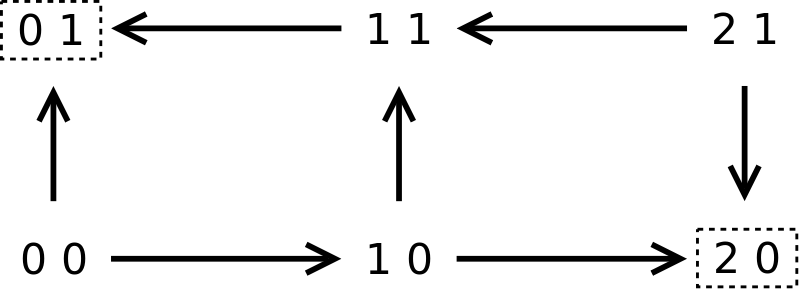
\includegraphics[width=7cm]{figs/graphe-d-etats}
  \caption{Le graphe d'états obtenu à partir du réseau de régulation de la figure~\ref{rrg-ex-parametrisation} \cite{richard-comet-bernot-08}. Chaque état est un couple du niveau d'expression des gènes $a$ et $b$, dans cet ordre.}
  \label{rrg-graphe-d-etats}
\end{figure}

Les graphes d'états offrent un outil efficace pour l'étude des réseaux de régulation. Cependant, il est important de noter à ce stade que la génération d'un graphe d'états est soumise à l'explosion combinatoire du nombre de ses états. En effet, l'ajout d'une variable dans le graphe d'interaction aura pour double conséquence :
\begin{itemize}
  \item d'ajouter un niveau d'expression à prendre en compte,
  \item de potentiellement faire augmenter le plafond d'une partie des autres gènes déjà présents dans le graphe d'interaction.
\end{itemize}
Ces deux éléments ont pour conséquence directe l'augmentation de la taille de graphe d'états, et peuvent entraîner des problèmes de mémoire et de temp d'exécution.

\section{Quelques définitions supplémentaires}
Certaines structures fréquemment rencontrées au sein des graphes d'états asynchrones obtenus par cette méthode sont décrites dans \cite{richard-comet-bernot-08}. Elles seront définies et expliquées dans la suite, et quelques théorèmes les concernant seront aussi donnés. Dans toute cette partie, on considère un réseau de régulation $N = (G ; \mathcal{K})$ dont $G$ est le graphe d'interaction et $\mathcal{K}$ la paramétrisation, et on appelle $\mathcal{S}_N$ son graphe d'états asynchrone.

\begin{definition}[Domaine piège]
Un \emph{domaine piège} de $\mathcal{S}_N$ est un sous-ensemble $T$ des n\oe uds du graphe tel que pour toute transition $x \rightarrow y$ dans $\mathcal{S}_N$, si $x \in T$, alors $y \in T$.
\end{definition}
D'après cette définition, un domaine piège est donc un sous-ensemble de configurations du système dont on ne peut sortir. Tout graphe d'états contient au moins un cas particulier de domaine piège, qui est l'ensemble de tous ses états.

\begin{definition}[Attracteur]
Un \emph{attracteur} de $\mathcal{S}_N$ est un domaine piège qui ne contient pas d'autre domaine piège que lui-même.
\end{definition}
La notion d'attracteur restreint celle de domaine piège en le caractérisant de plus petit domaine piège du point de vue de la relation d'inclusion. On peut donner quelques propriétés intéressantes concernant les attracteurs.

\begin{propriete}[Propriétés sur les attracteurs]~
\begin{itemize}
  \item Les attracteurs sont en fait les composantes fortement connexes du graphe (car si deux éléments $x$ et $y$ appartiennent au même attracteur, alors il existe un chemin de $x$ à $y$ et un chemin de $y$ à $x$).
  \item Tout graphe d'états contient au moins un attracteur (car il contient au moins un domaine piège).
  \item Les attracteurs sont mutuellement disjoints.
  \item Depuis tout état du graphe, il existe au moins un chemin conduisant à un attracteur.
\end{itemize}
\end{propriete}

\begin{definition}[État stable]
Un état puits (\textit{i.e.} qui ne possède aucun arc sortant) de $\mathcal{S}_N$ est appelé \emph{état stable}.
\end{definition}

Un état stable est un cas particulier d'attracteur (et donc de domaine piège) qui contient un seul élément. Lorsqu'un état stable est atteint, le système n'est plus en mesure d'évoluer. Les états stables d'un réseau de régulation peuvent être la conséquence de la \og victoire \fg{} de l'expression d'un ensemble de gènes sur un autre, ce dernier ne pouvant plus prendre le dessus. La figure~\ref{rrg-graphe-d-etats} contient deux attracteurs, entourés en pointillés ; ils modélisent le fait que l'un ou l'autre des deux gènes a gagné un niveau d'expression suffisant pour ne plus subir l'influence de l'autre gène.

Un attracteur composé de plus d'un seul élément (par opposition à un état stable) est appelé qualifié de \emph{cyclique}. Cette dénomination traduit le fait qu'un attracteur qui n'est pas un état stable contient nécessairement un cycle. Ce type d'attracteur peut potentiellement modéliser tout type de comportement oscillant d'un système.
